\todo{Put an image of the PCB here}

While the various cores of the genetics pipeline are the central components of the Barricelli system, the system itself would be little more than a simulation on some developer board without the printed circuit board (PCB) connecting all the components.
Designing the PCB and soldering components onto it are therefore important aspects of the development process of the Barricelli system.

In this chapter the PCB is presented.
The design and production processes are detailed.
Explanations are provided for why certain components were chosen.
And encountered problems and their workarounds are presented.

\section {Design choices}

\subsection{IO devices} \label{pcb:design-choices:ss:IO_devices}
USB
For usb interface we chosed the micro-usb. 
The reason for this is that the size of the assosiated hardware is much smaller.
In the design we also made circuts to prevent unwanted effects like electrostatic discharge, and circuts to prevent the signals from picking up unwanted noice from the background or from crosstalk.
Of course we also added neccessary resistances to prevent shortcircuting.

SD
We talked about using micro-sd cards, but because it was harder to find any guidlines on how to use/implement it we decided to use the normal SD interface.
In the SD interface, there are several protocols used for communication. 
However for this project we use the mode called "SPI bus mode", which is the interface that is used by the microcontroller.  
The SPI or "serial peripheral interface" is a scheme where you use a syncronized master-slave configuration or relation to communicate with the IO-devices. 
The goal with this choice is to have better compatibillity with the microcontroller.



\subsection{communication} \label{pcb:design-choices:ss:internal_communication}

\subsection{Memory} \label{pcb:design-choices:ss:memory}

 \label{pcb:section:design_choices}

\section {Power supply}

%% Add a picture of the power supply

As our requirements for the power supply were quite simmilar to the requirements of earlier projects from the subject.
The power supply from the Festiva Lente system was reused in our system.
This power supply have been used for many years, with small changes improving the behavior and performance of the power supply.
To avoid introducing new problems, reusing this power supply was a safe choice.
The barricelli system does however not require any 2.5 volt or 5 volt power.
As a result of this, these parts of the power supply have been removed in our system, and only 12 volt, 3.3 volt and 1.2 volt power is available in our system.

-insert picture here?

 \label{pcb:section:power_supply}

\section {Power plane}

 \label{pcb:section:power_plane}

\section{Footprints}
This section details how various footprints for components used in the project were obtained.

\subsection{Obtaining footprints}
Once a type of component has been decided upon for a project a specific instance of said component must be decided upon.
In order for said component to fit onto the PCB and properly function, its footprint, must be placed somewhere on the PCB.
The footprint is a kind of blueprint containing a component's outline and pads.

Obtaining a footprint for a component typically involves creating one manually or using a wizard based on the information contained in the component's datasheet.
Some manufacturers make footprints for their components available on their websites, however they might not be available in a format that is understandable by whatever PCB design suite that is employed in the current project.
Altium Designer (version 13.3) feature a browsable database of footprints for various components, all of which can be used immediately in any Altium project.

If a component's footprint is not readily available it has to be created manually.
The most important aspect of this process is to obtain the component's technical datasheet and examine it for a description of the component's package and dimensions.
This is sometimes labeled as an outline drawing, suggested land pattern (suggested pad size) or package outline.
It is important to notice what system the supplied measurements are in, as mixing for example imperial and metric units in a project could lead to unforseen incompatabilities.
Once one gets a hang of Altium PCB editor it takes surprisingly little time to create a footprint.

For components with standarized packages, Altium has an IPC compliant footprint wizard that generates footprints for a component given its package type and some package specific measurements available in the component's datasheet.

Note that the pads in the footprints should be slightly larger than the component's pins to make soldering easier.

\paragraph{USB}

the footprint for the micro-usb was found in the altium libary. 

\todo{kan vi kutte denne?}
\todo{as we can see in the picture, the usb have 4 pins that it uses. pin 1 is where the signal goes and.....}

\paragraph{SD}

The footprint for the SD-card was designed by the group. The reason for this was that appearently the sd-card interface is not standardized, so that 
every manufacturer have their own design on the receptacles. 

\todo{kan vi kutte denne?}

\todo{FIND THIS PICTURE: the picture shows the interface of the SD card. the different pins that can be seen on the picture are a part of the standardized SD-protocol that every manufacturer have to follow...}

 \label{pcb:section:footprints}

\section{Budget} \label{section:budget}
In this section you will find a dream that's not very sublime.
But rather the justly costs of one board produced.
and some other stuff
like how much wait we don't know how much it cost to produce the actual pcb?
lol
\todo{How much did PCB production cost?}
 \label{pcb:section:budget}

\section {Process}

Here we will introduse the design process.

\subsection{System design} \label{pcb:process:ss:system_design}

Here we will talk about how the system itself is designed on a logical level.

\subsection{PCB design and routing} \label{pcb:process:ss:pcb_design_and_soldering}

Here we will talk about how the design was transfered to the PCB, what problems were discovered in this process and how they were solved.

\subsection{Soldering} \label{pcb:process:ss:soldering}

Here we will talk about the soldering process and how we worked with that.
This will not cover major problems that needed a workaround (They are covered in their own chapter), but rather the challenges we experienced in the soldering process.
 \label{pcb:section:process}

\section {Problems and workaround}
Here we will talk about various problems we discovered during the soldering process, and how we found ways to workaround them.
We expect that there will be some things that may be possible to work around in code on the microcontroller, and other parts that require hardware fixes.
There might also be problems that cause parts of the board to not function.

\subsection{ Power connector footprint }

The footprint of the power connector had three pairs of holes instead of a milled groove.
This caused the connector to not fit in the footprint.
This was however solved by cutting away the parts of the connector that did not fit on the PCB using pliers.
The result worked fine, and it's hard to spot that the power connector is modified if you do not have a correctly mounted connector as a reference.

\subsection{ FPGA to SCU bus routing }

Because of an error made during the routing of the board, the header pin for FPGA\_ENABLE is not connected to any FPGA pins.
This error can be corrected by using one of our spare FPGA lines available on headers.
A wire was pulled from FPGA\_HEADER78 to the header from the SCU, and this header cable allowed us to run the rest of the bus as planed.

\begin{figure}[H]
\centering
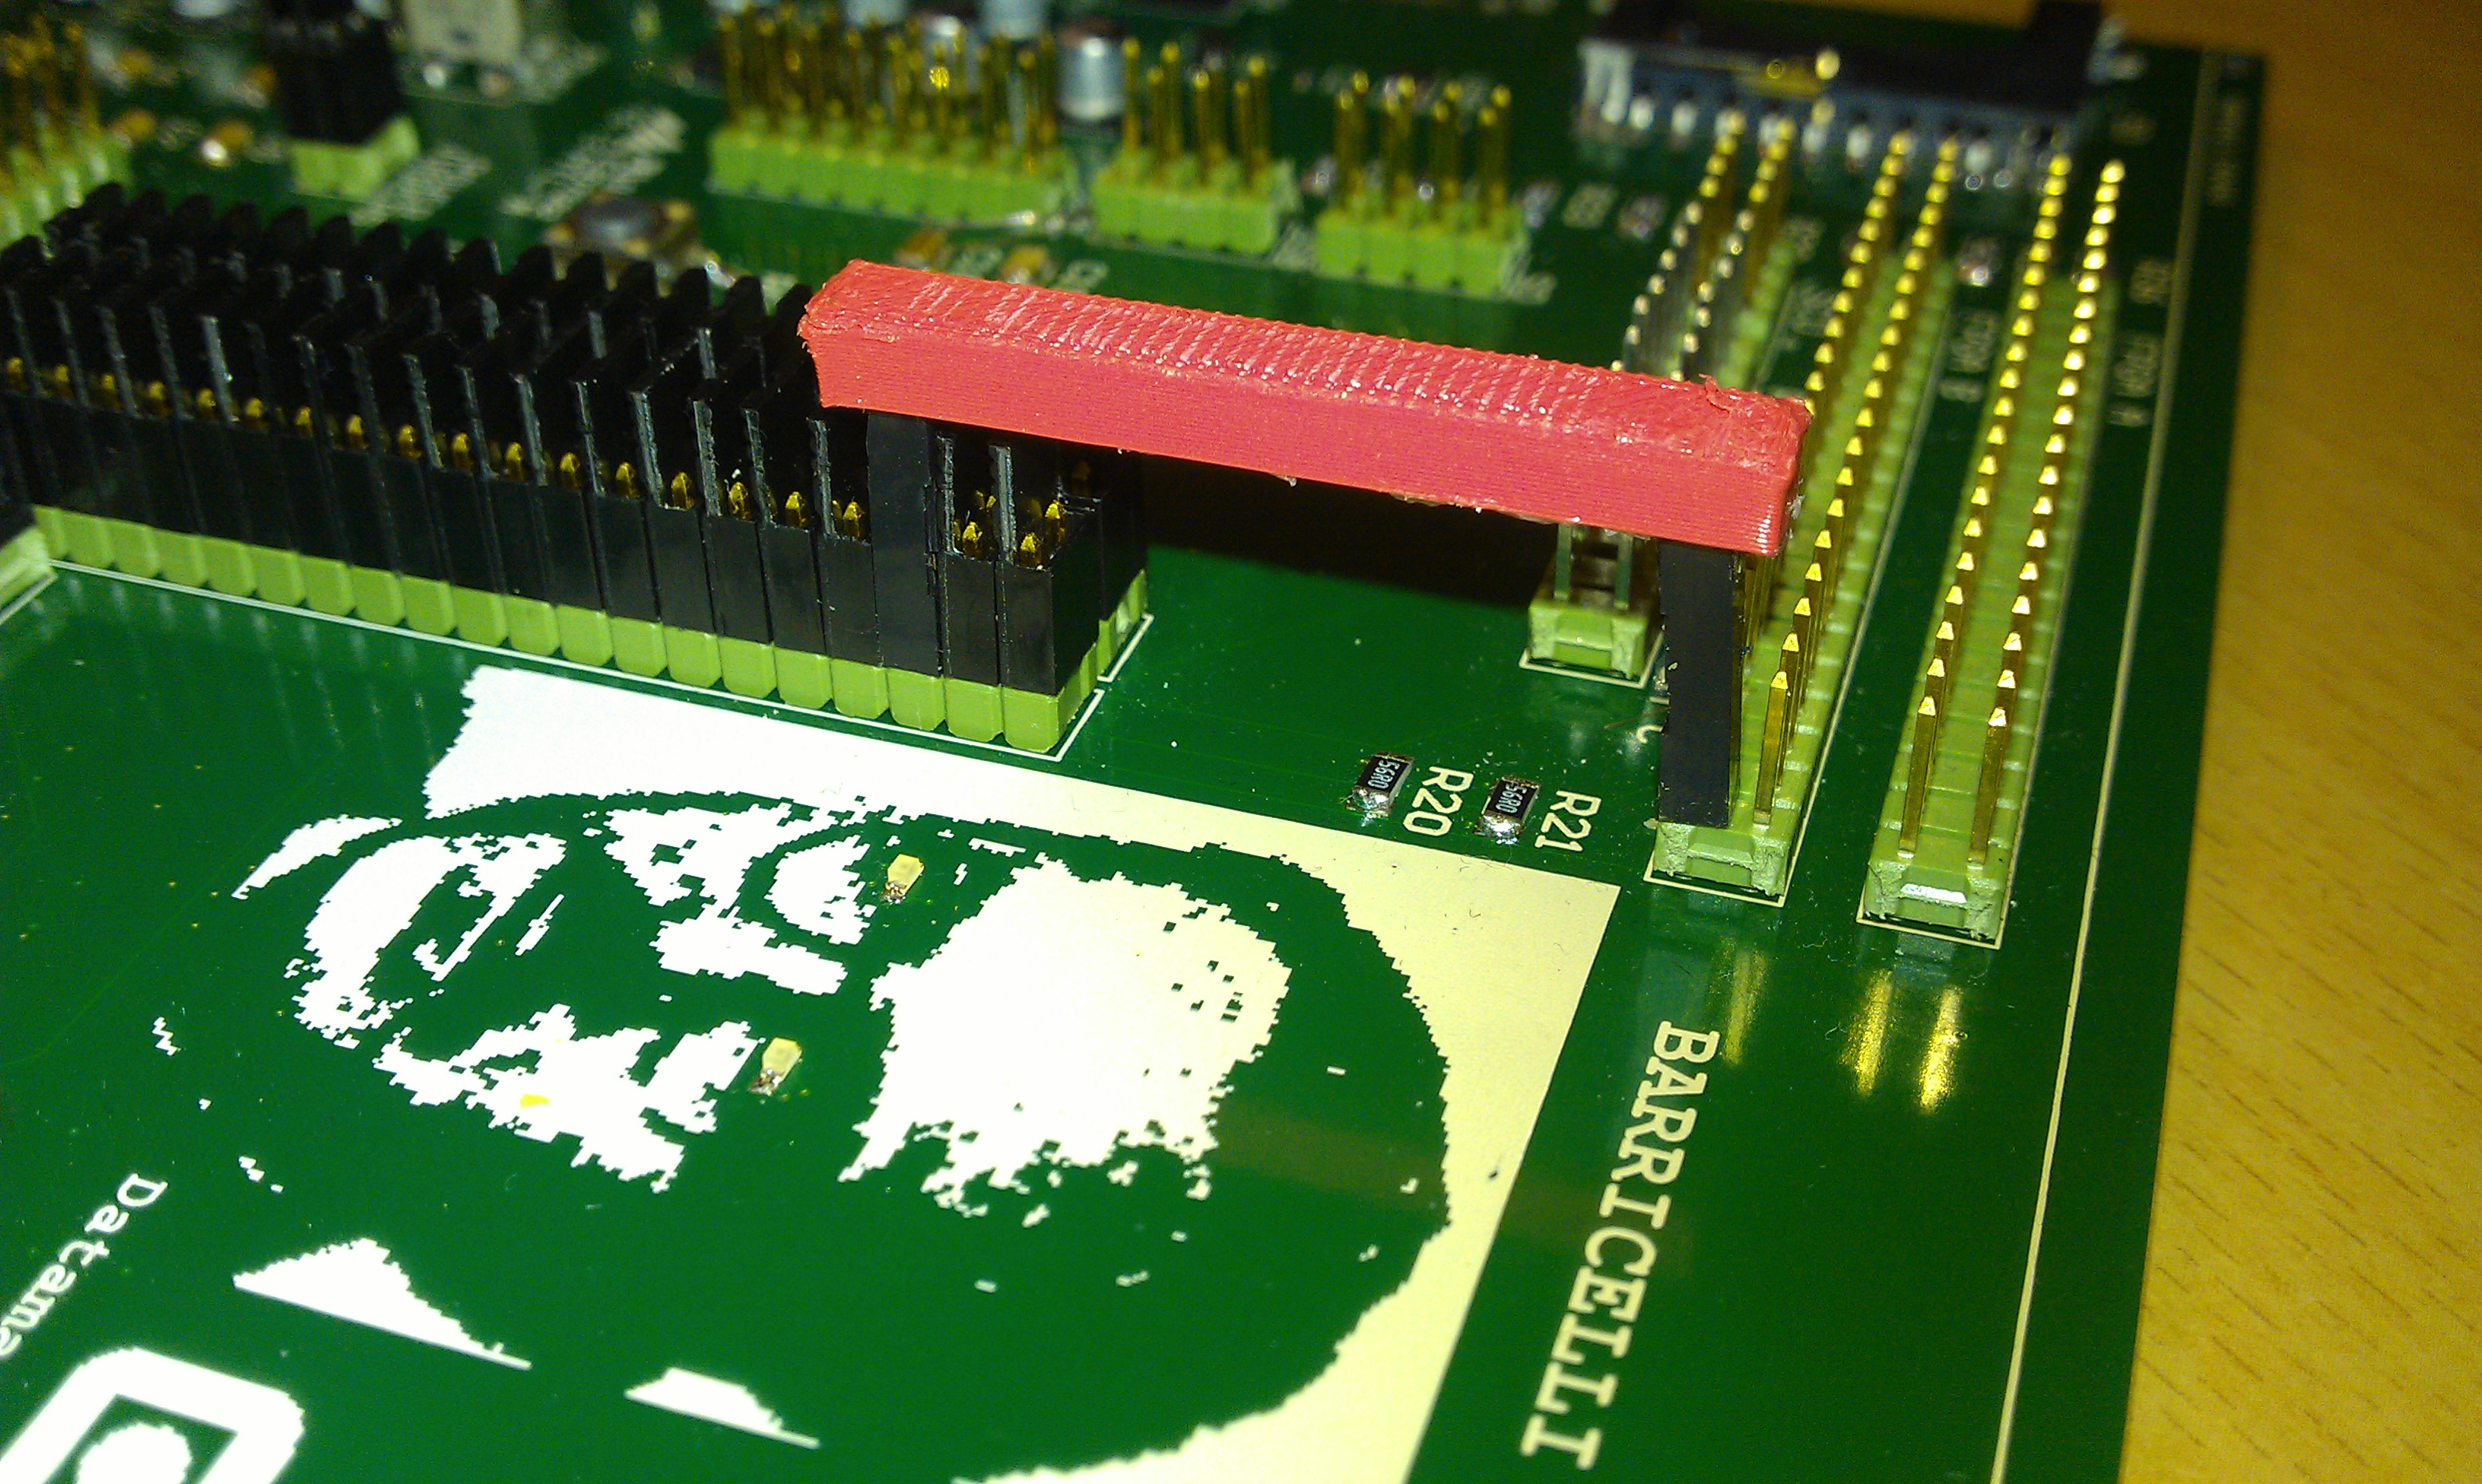
\includegraphics[width=10cm,keepaspectratio]{pcb/enable_hack.jpg}
\caption{For aesthetic appeal we 3D printed a bridge for the wire to run in}
\label{figure:vreghack}
\end{figure}

\subsection{ USB port }

\begin{figure}
\centering
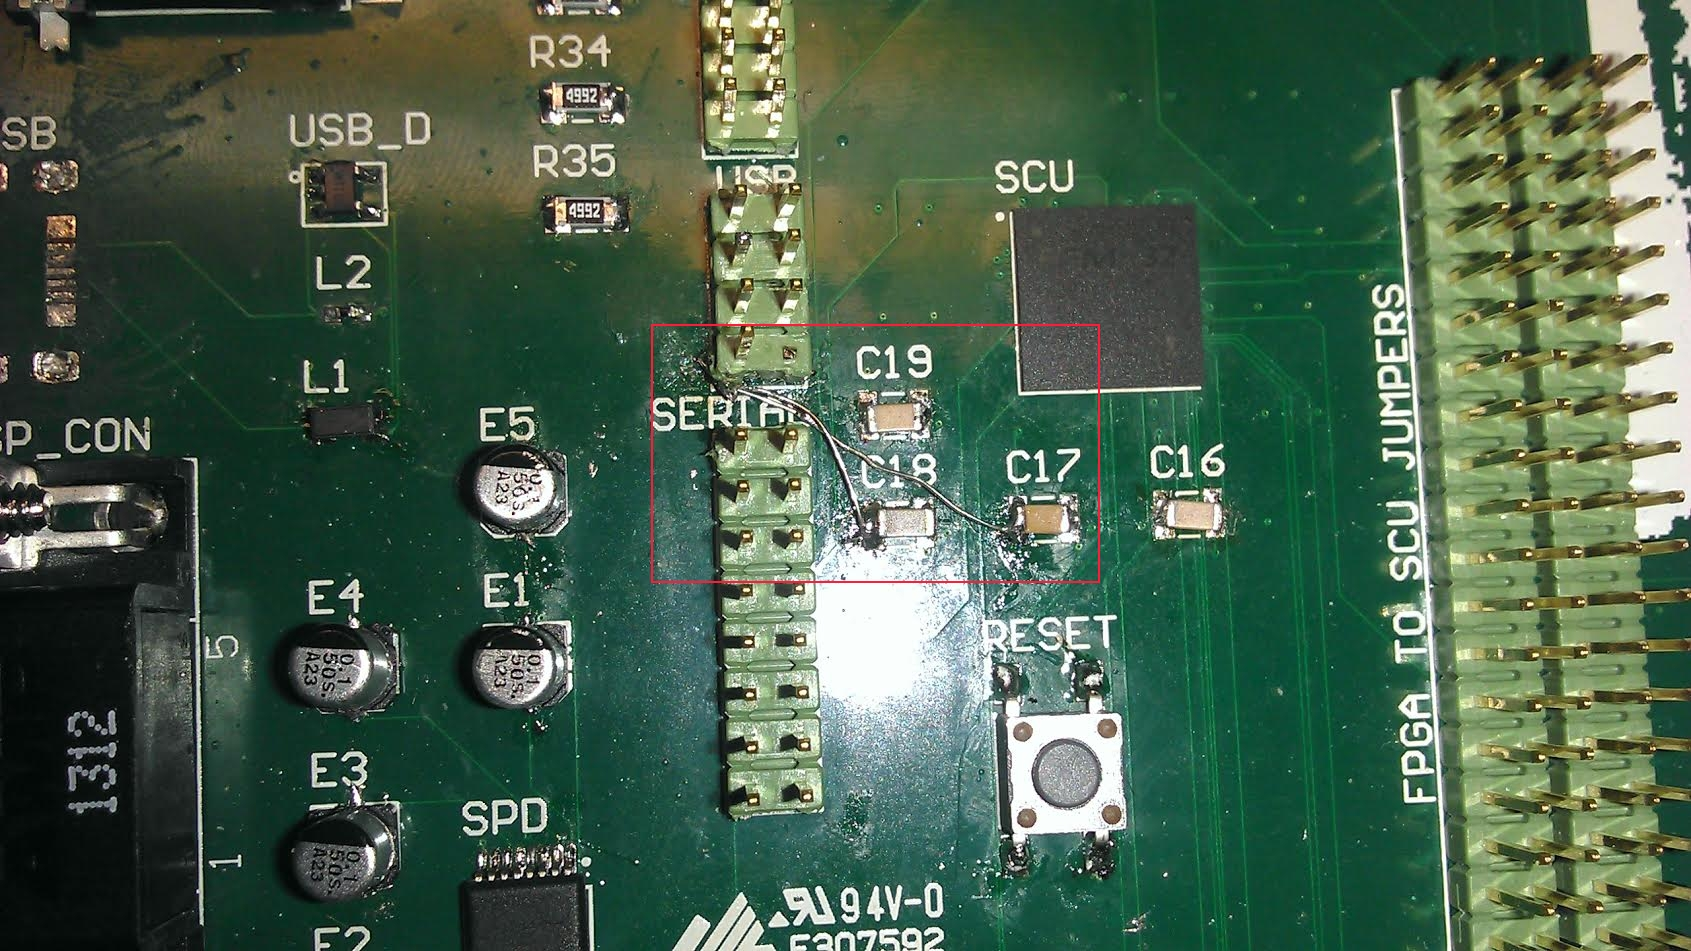
\includegraphics[width=10cm,keepaspectratio]{pcb/vreghack.jpg}
\caption{The figure shows the ``hack'' that were made on the PCB in an attempt to fix the USB. Sadly the board were accidentally shortcircuted and died before this the hack could be fully verified to be working}
\label{figure:vreghack}
\end{figure}

When the PCB came back from production, it was discovered that the USB was not connected to the microcontroller
according to the recommended specifications from the manufacturer of the microcontroller. 
The problem was that the signals USB\_VBUS and USB\_VREGI were not connected to the VBUS-pin on the USB receptacle. This was fixed by soldering copper wires on the capacitors designated as C18 and C17 to USB-HEADER2 (called VBUS\_ENABLE in the schematics).
According to tests performed on the PCB before and after this work-around, the problem was fixed successfully.
 \label{pcb:section:problems_and_workaround}

